\documentclass[11pt]{article}

\usepackage[margin=1in]{geometry}
\usepackage{graphicx}
\usepackage{booktabs}
\usepackage{amsmath}
\usepackage{float}
\usepackage{listings}
\usepackage{xcolor}
\usepackage{subcaption}

\graphicspath{{../results/auto_mpg/}{../results/concrete/}{../results/airfoil/}}

\lstset{
    basicstyle=\ttfamily\scriptsize,
    breaklines=true,
    breakatwhitespace=true,
    frame=single,
    columns=fullflexible
}

\makeatletter
\newcommand{\resizetableifneeded}[1]{%
    \sbox0{#1}%
    \ifdim\wd0>\textwidth
        \resizebox{\textwidth}{!}{\usebox0}%
    \else
        \usebox0
    \fi
}
\makeatother

\title{Project 1: Exploratory Data Analysis and Simple Regression}
\author{Seth Cohen}
\date{\today}

\begin{document}
\maketitle

\section*{Overview}
This report presents an exploratory data analysis (EDA) and simple (univariate)
linear regression study on three datasets from the UCI Machine Learning
Repository: Auto MPG, Concrete Compressive Strength, and Airfoil Self-Noise.
For each dataset we (1) describe preprocessing steps, (2) report statistical
summaries for every feature, (3) compute a correlation matrix and heatmap,
and (4) fit a simple linear regression model, $y = b_0 + b_1 x$, for the two
predictor features most strongly correlated with the target, using both
\textbf{ScalaTion} and Python's \textbf{Statsmodels}.

\clearpage
\section{Auto MPG Dataset}

\subsection{Description}
The Auto MPG dataset relates a car's fuel economy (miles per gallon, mpg) to
seven engine and body characteristics. After cleaning, it contains 392 rows
and 8 columns.

\subsection{Preprocessing}
The raw \texttt{auto-mpg.data} file is whitespace-delimited and contains 398
rows and 9 columns, the last of which (\texttt{car name}) is a unique string
identifier for each car and is not useful as a regression feature. Six rows
have a missing (\texttt{?}) value for \texttt{horsepower}; these were dropped
during the conversion to CSV, along with the \texttt{car name} column, leaving
392 rows and 8 numeric columns (\texttt{mpg}, \texttt{cylinders},
\texttt{displacement}, \texttt{horsepower}, \texttt{weight},
\texttt{acceleration}, \texttt{model\_year}, \texttt{origin}) exactly matching
the expected shape. No further outlier removal was performed: an IQR-rule
check flags 10 \texttt{horsepower} values and 11 \texttt{acceleration} values
as statistical outliers, but these correspond to genuinely high-performance
or economy vehicles rather than data errors, so they were kept.

\subsection{Statistical Summary}
\resizetableifneeded{\begin{tabular}{lrrrrrrrr}
\toprule
Feature & count & mean & std & min & 25\% & 50\% & 75\% & max \\
\midrule
mpg & 392.000 & 23.446 & 7.805 & 9.000 & 17.000 & 22.750 & 29.000 & 46.600 \\
cylinders & 392.000 & 5.472 & 1.706 & 3.000 & 4.000 & 4.000 & 8.000 & 8.000 \\
displacement & 392.000 & 194.412 & 104.644 & 68.000 & 105.000 & 151.000 & 275.750 & 455.000 \\
horsepower & 392.000 & 104.469 & 38.491 & 46.000 & 75.000 & 93.500 & 126.000 & 230.000 \\
weight & 392.000 & 2977.584 & 849.403 & 1613.000 & 2225.250 & 2803.500 & 3614.750 & 5140.000 \\
acceleration & 392.000 & 15.541 & 2.759 & 8.000 & 13.775 & 15.500 & 17.025 & 24.800 \\
model\_year & 392.000 & 75.980 & 3.684 & 70.000 & 73.000 & 76.000 & 79.000 & 82.000 \\
origin & 392.000 & 1.577 & 0.806 & 1.000 & 1.000 & 1.000 & 2.000 & 3.000 \\
\bottomrule
\end{tabular}}

\subsection{Correlation Analysis}
\begin{tabular}{lr}
\toprule
Feature & Correlation with target \\
\midrule
weight & -0.8322 \\
displacement & -0.8051 \\
horsepower & -0.7784 \\
cylinders & -0.7776 \\
model\_year & 0.5805 \\
origin & 0.5652 \\
acceleration & 0.4233 \\
\bottomrule
\end{tabular}

Table~\ref{tab:auto-mpg-full-corr} gives the complete feature-by-feature
correlation matrix, and Figure~\ref{fig:auto-mpg-heatmap} shows the
corresponding heatmap.

\begin{table}[H]
    \centering
    \caption{Full correlation matrix, Auto MPG dataset.}
    \label{tab:auto-mpg-full-corr}
    \resizetableifneeded{\begin{tabular}{lrrrrrrrr}
\toprule
Feature & mpg & C & D & H & W & A & MY & O \\
\midrule
mpg & 1.00 & -0.78 & -0.81 & -0.78 & -0.83 & 0.42 & 0.58 & 0.57 \\
cylinders & -0.78 & 1.00 & 0.95 & 0.84 & 0.90 & -0.50 & -0.35 & -0.57 \\
displacement & -0.81 & 0.95 & 1.00 & 0.90 & 0.93 & -0.54 & -0.37 & -0.61 \\
horsepower & -0.78 & 0.84 & 0.90 & 1.00 & 0.86 & -0.69 & -0.42 & -0.46 \\
weight & -0.83 & 0.90 & 0.93 & 0.86 & 1.00 & -0.42 & -0.31 & -0.59 \\
acceleration & 0.42 & -0.50 & -0.54 & -0.69 & -0.42 & 1.00 & 0.29 & 0.21 \\
model\_year & 0.58 & -0.35 & -0.37 & -0.42 & -0.31 & 0.29 & 1.00 & 0.18 \\
origin & 0.57 & -0.57 & -0.61 & -0.46 & -0.59 & 0.21 & 0.18 & 1.00 \\
\bottomrule
\end{tabular}}\\[4pt]
    {\footnotesize C=cylinders; D=displacement; H=horsepower; W=weight; A=acceleration; MY=model\_year; O=origin}
\end{table}

\begin{figure}[H]
    \centering
    
\includegraphics[width=0.75\textwidth]{corr_heatmap.png}
    \caption{Correlation heatmap for the Auto MPG dataset.}
    \label{fig:auto-mpg-heatmap}
\end{figure}

\subsection{Top Two Predictor Variables}
Based on the correlation analysis above, the two predictors most strongly
correlated (by magnitude) with \texttt{mpg} are \texttt{weight}
($r=-0.83$) and \texttt{displacement} ($r=-0.81$), ahead of
\texttt{horsepower} ($r=-0.78$) and \texttt{cylinders} ($r=-0.78$). These
two features are used consistently in both the ScalaTion and Statsmodels
simple regressions below.

\subsection{Simple Regression Models}

\subsubsection*{Feature: weight}
\textbf{ScalaTion fit report:}
\lstinputlisting{listings/auto_mpg_weight_scalation.txt}

\textbf{Statsmodels fit report:}
\lstinputlisting{../results/auto_mpg/ols_summary_weight.txt}

\textbf{Summary statement:} Both tools agree exactly on
$\hat{y} = 46.2165 - 0.0076\,x$. Each additional pound of vehicle weight is
associated with a decrease of about 0.0076 mpg; the model explains 69.3\%
of the variance in mpg ($R^2=0.6926$, adj.\ $R^2=0.6918$), and the slope is
highly statistically significant ($F=878.83$, $p<0.001$).

\begin{figure}[H]
    \centering
    \begin{subfigure}{0.48\textwidth}
        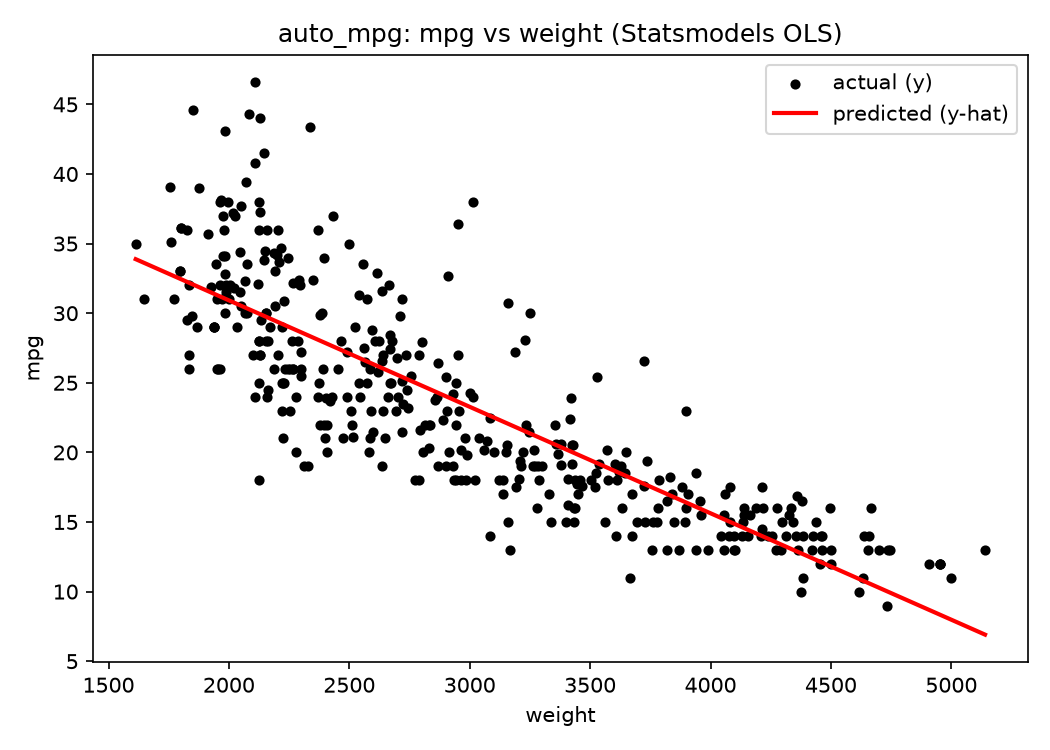
\includegraphics[width=\textwidth]{fit_vs_actual_weight.png}
        \caption{Statsmodels}
    \end{subfigure}
    \begin{subfigure}{0.48\textwidth}
        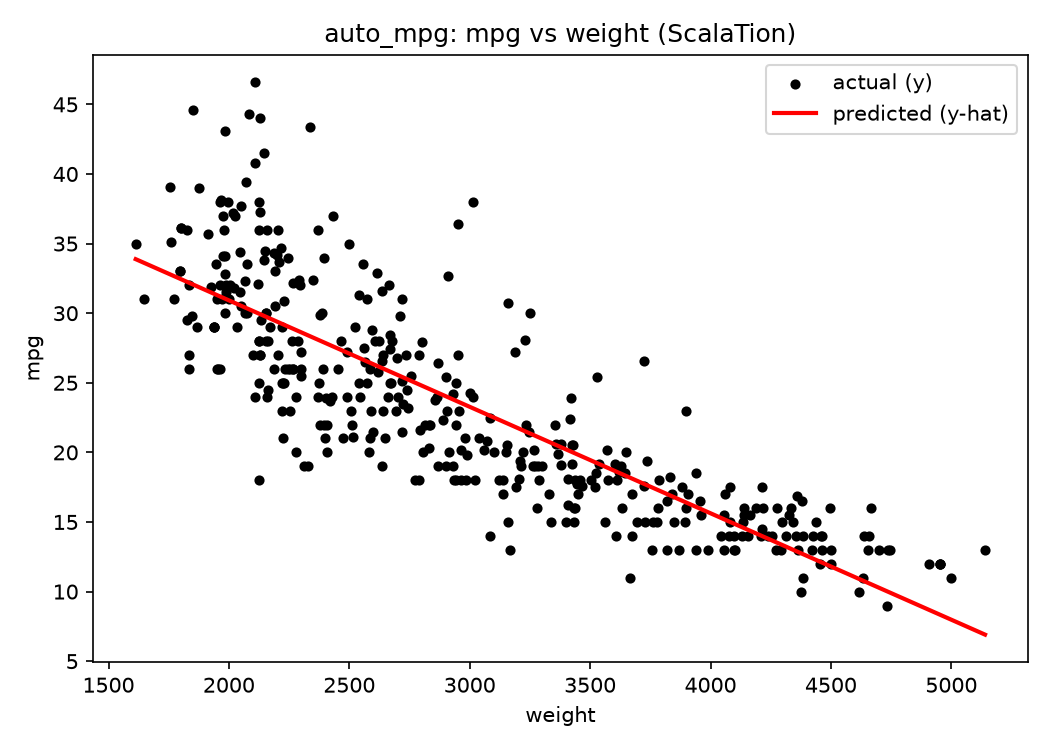
\includegraphics[width=\textwidth]{scalation_fit_vs_actual_weight.png}
        \caption{ScalaTion}
    \end{subfigure}
    \caption{mpg vs.\ weight: actual (black) and predicted (red) values.}
\end{figure}

\subsubsection*{Feature: displacement}
\textbf{ScalaTion fit report:}
\lstinputlisting{listings/auto_mpg_displacement_scalation.txt}

\textbf{Statsmodels fit report:}
\lstinputlisting{../results/auto_mpg/ols_summary_displacement.txt}

\textbf{Summary statement:} Both tools agree exactly on
$\hat{y} = 35.1206 - 0.0601\,x$. Each additional cubic inch of engine
displacement is associated with a decrease of about 0.06 mpg; the model
explains 64.8\% of the variance in mpg ($R^2=0.6482$, adj.\ $R^2=0.6473$),
and the slope is highly statistically significant ($F=718.68$, $p<0.001$).

\begin{figure}[H]
    \centering
    \begin{subfigure}{0.48\textwidth}
        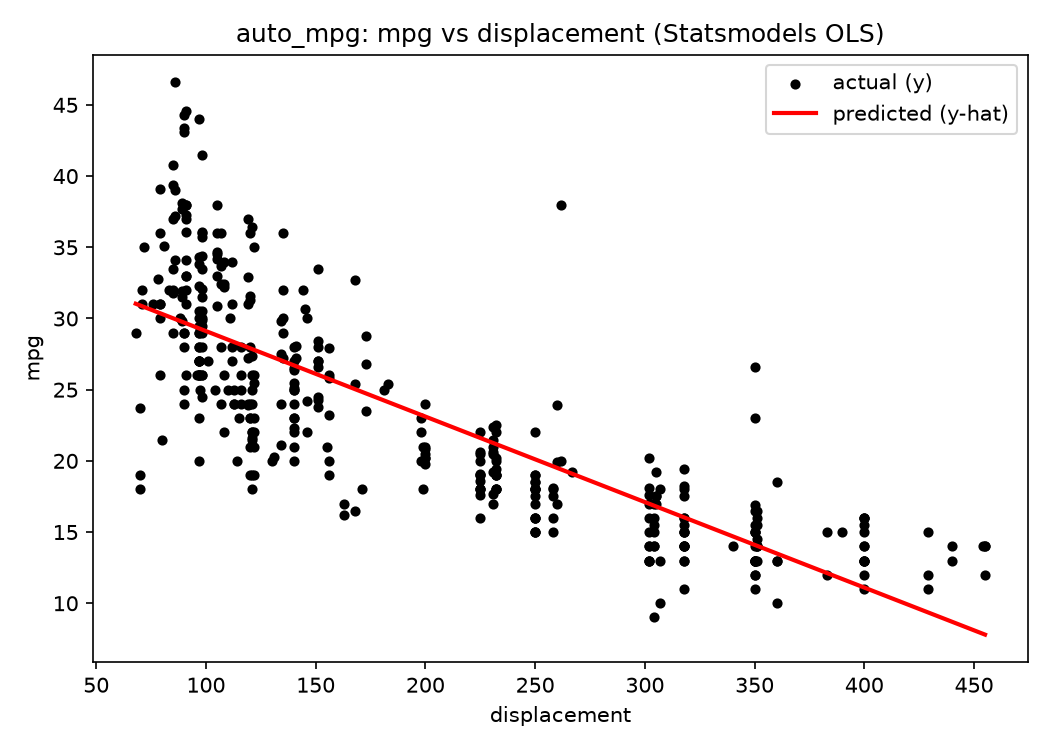
\includegraphics[width=\textwidth]{fit_vs_actual_displacement.png}
        \caption{Statsmodels}
    \end{subfigure}
    \begin{subfigure}{0.48\textwidth}
        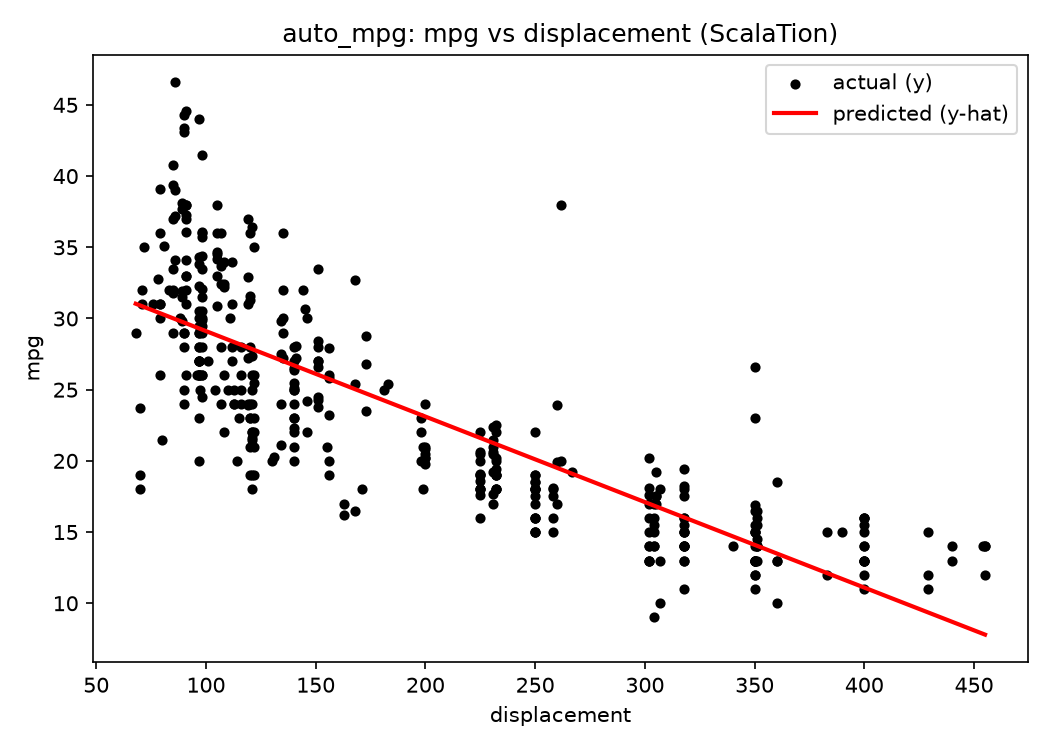
\includegraphics[width=\textwidth]{scalation_fit_vs_actual_displacement.png}
        \caption{ScalaTion}
    \end{subfigure}
    \caption{mpg vs.\ displacement: actual (black) and predicted (red) values.}
\end{figure}

\subsection{Discussion}
Both predictors yield a strong, statistically significant negative linear
relationship with fuel economy: heavier cars with larger engines get fewer
miles per gallon, consistent with basic physics (more mass and displacement
require more fuel to move). \texttt{weight} is the single best univariate
predictor ($R^2 \approx 0.69$), narrowly ahead of \texttt{displacement}
($R^2 \approx 0.65$); the two are themselves highly correlated ($r=0.93$,
see heatmap), so they capture overlapping information about vehicle size.
ScalaTion and Statsmodels produce numerically identical coefficients and
$R^2$ values, as expected for ordinary least squares fit on the same data --
this agreement is a useful sanity check that both toolchains are correctly
configured. Neither univariate model fully explains \texttt{mpg}
($R^2 < 0.70$), suggesting a multiple regression using several of these
correlated features together (or a nonlinear model) would fit noticeably
better.

\clearpage
\section{Concrete Compressive Strength Dataset}

\subsection{Description}
This dataset relates the compressive strength of concrete (MPa) to the
proportions of its ingredients and its curing age. It contains 1030 rows and
9 columns (8 quantitative ingredient/age features plus the strength target).

\subsection{Preprocessing}
\begin{sloppypar}
The raw data ships as an Excel spreadsheet (\texttt{Concrete\_Data.xls}) with
verbose column headers. It was loaded with pandas, renamed to concise
snake\_case names (\texttt{cement}, \texttt{blast\_furnace\_slag},
\texttt{fly\_ash}, \texttt{water}, \texttt{superplasticizer},
\texttt{coarse\_aggregate}, \texttt{fine\_aggregate}, \texttt{age},
\texttt{concrete\_compressive\_strength}), and written out as a plain CSV.
The dataset has no missing values and no string columns, so no rows were
dropped; its cleaned shape (1030, 9) matches the documented dataset size
exactly. An IQR-rule check flags outliers in several columns (most
prominently \texttt{age}, with 59 flagged values, since age ranges from 1 to
365 days and is heavily right-skewed) -- these were kept, as they represent
valid experimental conditions rather than data-entry errors.
\end{sloppypar}

\subsection{Statistical Summary}
\resizetableifneeded{\begin{tabular}{lrrrrrrrr}
\toprule
Feature & count & mean & std & min & 25\% & 50\% & 75\% & max \\
\midrule
cement & 1030.000 & 281.166 & 104.507 & 102.000 & 192.375 & 272.900 & 350.000 & 540.000 \\
blast\_furnace\_slag & 1030.000 & 73.895 & 86.279 & 0.000 & 0.000 & 22.000 & 142.950 & 359.400 \\
fly\_ash & 1030.000 & 54.187 & 63.996 & 0.000 & 0.000 & 0.000 & 118.270 & 200.100 \\
water & 1030.000 & 181.566 & 21.356 & 121.750 & 164.900 & 185.000 & 192.000 & 247.000 \\
superplasticizer & 1030.000 & 6.203 & 5.973 & 0.000 & 0.000 & 6.350 & 10.160 & 32.200 \\
coarse\_aggregate & 1030.000 & 972.919 & 77.754 & 801.000 & 932.000 & 968.000 & 1029.400 & 1145.000 \\
fine\_aggregate & 1030.000 & 773.579 & 80.175 & 594.000 & 730.950 & 779.510 & 824.000 & 992.600 \\
age & 1030.000 & 45.662 & 63.170 & 1.000 & 7.000 & 28.000 & 56.000 & 365.000 \\
concrete\_compressive\_strength & 1030.000 & 35.818 & 16.706 & 2.332 & 23.707 & 34.443 & 46.136 & 82.599 \\
\bottomrule
\end{tabular}}

\subsection{Correlation Analysis}
\begin{tabular}{lr}
\toprule
Feature & Correlation with target \\
\midrule
cement & 0.4978 \\
superplasticizer & 0.3661 \\
age & 0.3289 \\
water & -0.2896 \\
fine\_aggregate & -0.1672 \\
coarse\_aggregate & -0.1649 \\
blast\_furnace\_slag & 0.1348 \\
fly\_ash & -0.1058 \\
\bottomrule
\end{tabular}

Table~\ref{tab:concrete-full-corr} gives the complete feature-by-feature
correlation matrix, and Figure~\ref{fig:concrete-heatmap} shows the
corresponding heatmap.

\begin{table}[H]
    \centering
    \caption{Full correlation matrix, Concrete Compressive Strength dataset.}
    \label{tab:concrete-full-corr}
    \resizetableifneeded{\begin{tabular}{lrrrrrrrrr}
\toprule
Feature & C & BFS & FA & W & S & CA & FA2 & age & CCS \\
\midrule
cement & 1.00 & -0.28 & -0.40 & -0.08 & 0.09 & -0.11 & -0.22 & 0.08 & 0.50 \\
blast\_furnace\_slag & -0.28 & 1.00 & -0.32 & 0.11 & 0.04 & -0.28 & -0.28 & -0.04 & 0.13 \\
fly\_ash & -0.40 & -0.32 & 1.00 & -0.26 & 0.38 & -0.01 & 0.08 & -0.15 & -0.11 \\
water & -0.08 & 0.11 & -0.26 & 1.00 & -0.66 & -0.18 & -0.45 & 0.28 & -0.29 \\
superplasticizer & 0.09 & 0.04 & 0.38 & -0.66 & 1.00 & -0.27 & 0.22 & -0.19 & 0.37 \\
coarse\_aggregate & -0.11 & -0.28 & -0.01 & -0.18 & -0.27 & 1.00 & -0.18 & -0.00 & -0.16 \\
fine\_aggregate & -0.22 & -0.28 & 0.08 & -0.45 & 0.22 & -0.18 & 1.00 & -0.16 & -0.17 \\
age & 0.08 & -0.04 & -0.15 & 0.28 & -0.19 & -0.00 & -0.16 & 1.00 & 0.33 \\
concrete\_compressive\_strength & 0.50 & 0.13 & -0.11 & -0.29 & 0.37 & -0.16 & -0.17 & 0.33 & 1.00 \\
\bottomrule
\end{tabular}}\\[4pt]
    {\footnotesize C=cement; BFS=blast\_furnace\_slag; FA=fly\_ash; W=water; S=superplasticizer; CA=coarse\_aggregate; FA2=fine\_aggregate; CCS=concrete\_compressive\_strength}
\end{table}

\begin{figure}[H]
    \centering
    
\includegraphics[width=0.8\textwidth]{corr_heatmap.png}
    \caption{Correlation heatmap for the Concrete Compressive Strength dataset.}
    \label{fig:concrete-heatmap}
\end{figure}

\subsection{Top Two Predictor Variables}
Based on the correlation analysis above, the two predictors most strongly
correlated with compressive strength are \texttt{cement} ($r=0.50$) and
\texttt{superplasticizer} ($r=0.37$), ahead of \texttt{age} ($r=0.33$) and
\texttt{water} ($r=-0.29$). These two features are used consistently in
both the ScalaTion and Statsmodels simple regressions below.

\subsection{Simple Regression Models}

\subsubsection*{Feature: cement}
\textbf{ScalaTion fit report:}
\lstinputlisting{listings/concrete_cement_scalation.txt}

\textbf{Statsmodels fit report:}
\lstinputlisting{../results/concrete/ols_summary_cement.txt}

\textbf{Summary statement:} Both tools agree exactly on
$\hat{y} = 13.4428 + 0.0796\,x$. Each additional kg/m$^3$ of cement is
associated with an increase of about 0.08 MPa in compressive strength; the
model explains only 24.8\% of the variance ($R^2=0.2478$, adj.\
$R^2=0.2471$), though the slope is highly statistically significant
($F=338.73$, $p<0.001$).

\begin{figure}[H]
    \centering
    \begin{subfigure}{0.48\textwidth}
        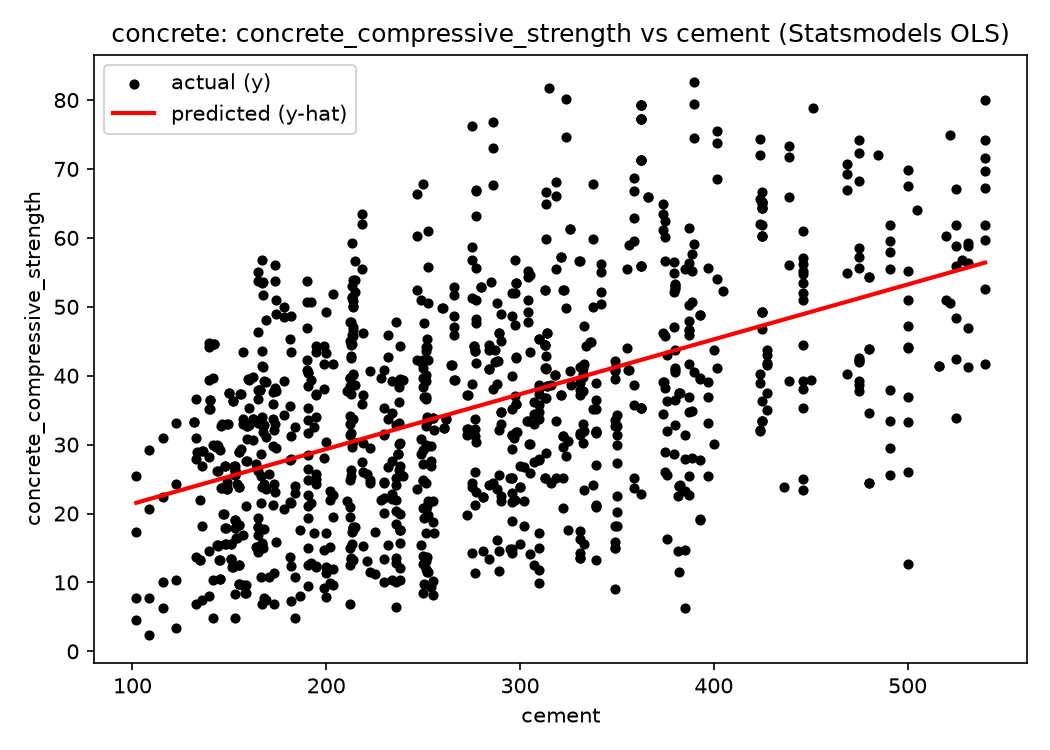
\includegraphics[width=\textwidth]{fit_vs_actual_cement.png}
        \caption{Statsmodels}
    \end{subfigure}
    \begin{subfigure}{0.48\textwidth}
        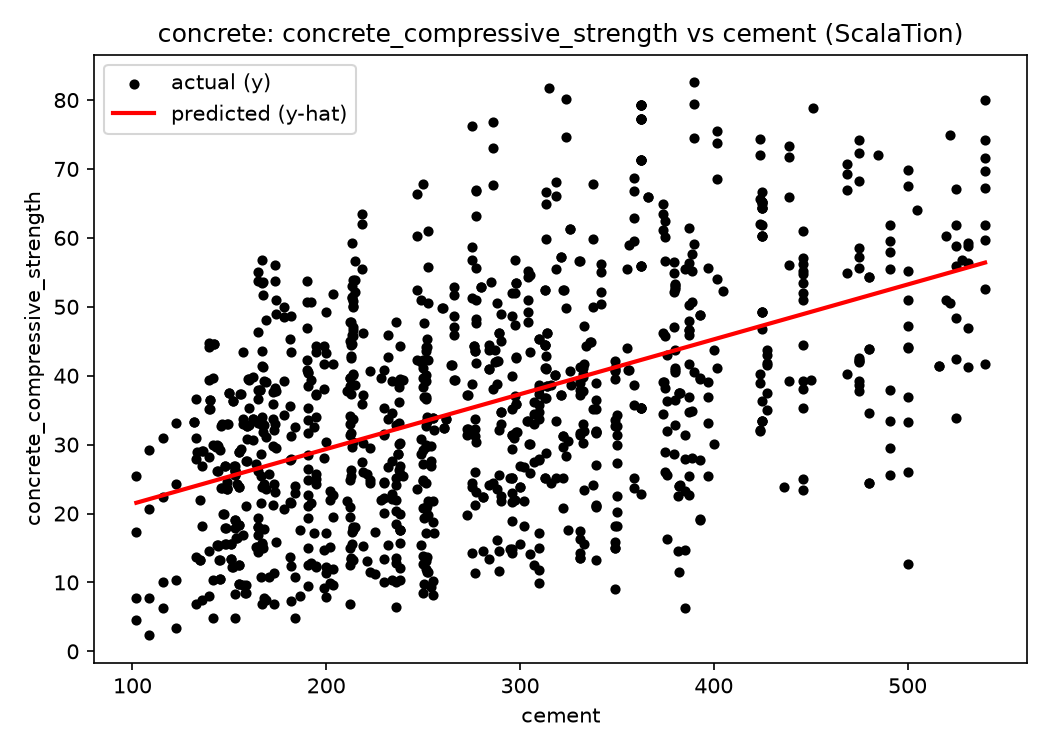
\includegraphics[width=\textwidth]{scalation_fit_vs_actual_cement.png}
        \caption{ScalaTion}
    \end{subfigure}
    \caption{Compressive strength vs.\ cement content: actual (black) and predicted (red) values.}
\end{figure}

\subsubsection*{Feature: superplasticizer}
\textbf{ScalaTion fit report:}
\lstinputlisting{listings/concrete_superplasticizer_scalation.txt}

\textbf{Statsmodels fit report:}
\lstinputlisting{../results/concrete/ols_summary_superplasticizer.txt}

\textbf{Summary statement:} Both tools agree exactly on
$\hat{y} = 29.4668 + 1.0239\,x$. Each additional kg/m$^3$ of
superplasticizer is associated with an increase of about 1.02 MPa in
compressive strength; the model explains only 13.4\% of the variance
($R^2=0.1340$, adj.\ $R^2=0.1332$), though the slope is highly
statistically significant ($F=159.11$, $p<0.001$).

\begin{figure}[H]
    \centering
    \begin{subfigure}{0.48\textwidth}
        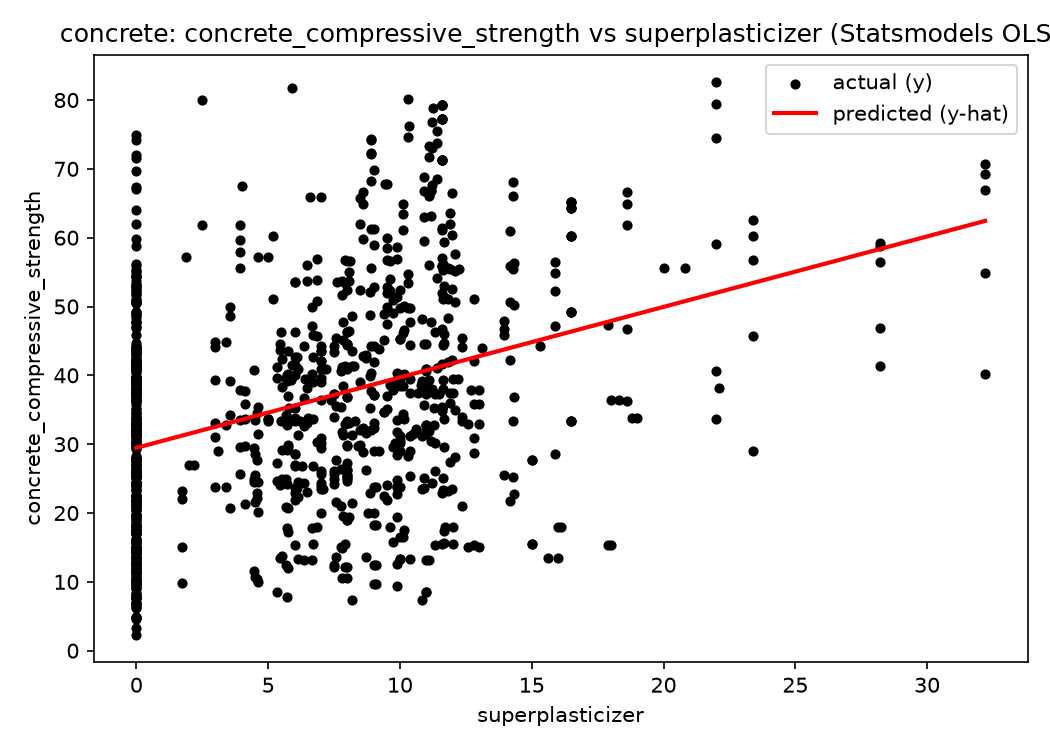
\includegraphics[width=\textwidth]{fit_vs_actual_superplasticizer.png}
        \caption{Statsmodels}
    \end{subfigure}
    \begin{subfigure}{0.48\textwidth}
        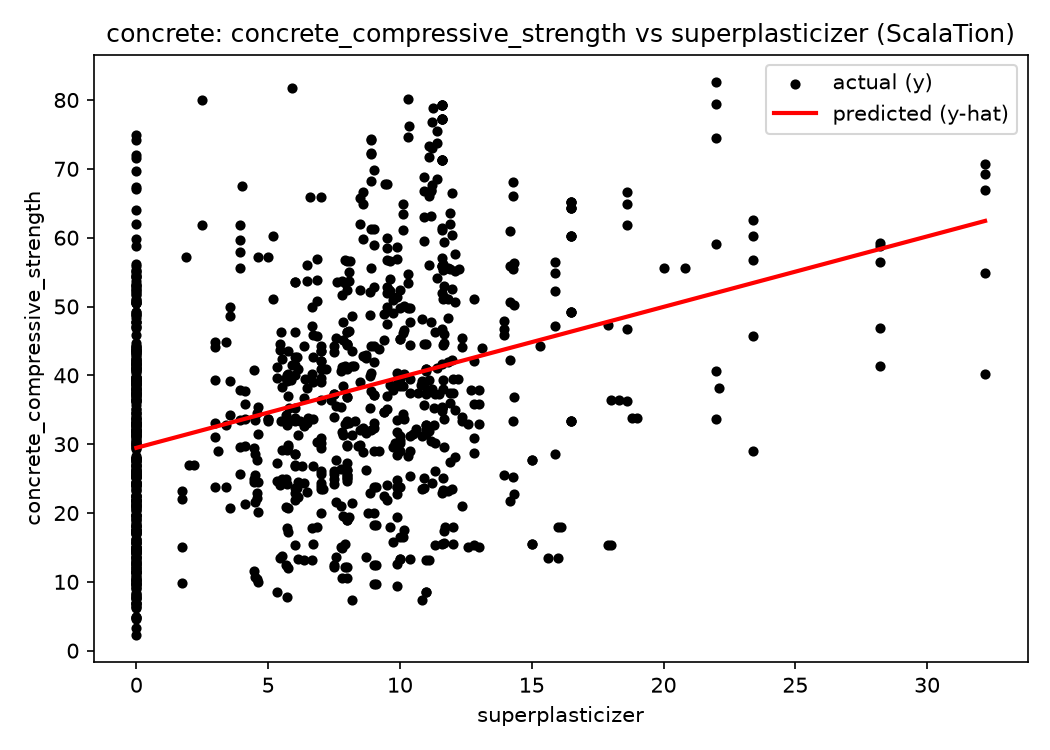
\includegraphics[width=\textwidth]{scalation_fit_vs_actual_superplasticizer.png}
        \caption{ScalaTion}
    \end{subfigure}
    \caption{Compressive strength vs.\ superplasticizer dosage: actual (black) and predicted (red) values.}
\end{figure}

\subsection{Discussion}
Compressive strength is a genuinely multivariate phenomenon -- it depends
simultaneously on the amounts of cement, water, various admixtures, and
curing age -- so no single ingredient explains most of the variance on its
own. \texttt{cement} content is the strongest univariate predictor, but it
only accounts for about 25\% of the variance ($R^2 = 0.25$), and
\texttt{superplasticizer} explains just 13\%. Both relationships are positive
and highly statistically significant, matching material-science expectations
(more cement binder and more superplasticizer, which improves workability at
low water content, both tend to increase strength), but the wide scatter
visible in the fit plots shows that a simple one-variable model is a poor
overall predictor here -- unlike Auto MPG, this dataset would benefit
substantially from multiple regression using all 8 ingredient/age features
together.

\clearpage
\section{Airfoil Self-Noise Dataset}

\subsection{Description}
This NASA dataset relates the scaled sound pressure level (decibels)
produced by airfoils in a wind tunnel to five aerodynamic and geometric
parameters. It contains 1503 rows and 6 columns.

\subsection{Preprocessing}
\begin{sloppypar}
The raw data ships as a tab-delimited \texttt{.dat} file with no header row.
It was converted directly to CSV, adding the column names \texttt{frequency},
\texttt{angle\_of\_attack}, \texttt{chord\_length},
\texttt{free\_stream\_velocity}, \texttt{suction\_side\_displacement\_thickness},
and \texttt{scaled\_sound\_pressure\_level} (the target) based on the
dataset's documentation. There are no missing values and no string columns,
so no rows were dropped, and the cleaned shape (1503, 6) matches the
documented size exactly. An IQR-rule check flags a substantial number of
outliers in \texttt{frequency} (86), \texttt{angle\_of\_attack} (30), and
\texttt{suction\_side\_displacement\_thickness} (124) -- these reflect the
wide range of physical test conditions used in the wind-tunnel experiments
(frequency spans 200--20{,}000 Hz) rather than data-quality problems, so all
rows were retained.
\end{sloppypar}

\subsection{Statistical Summary}
\resizetableifneeded{\begin{tabular}{lrrrrrrrr}
\toprule
Feature & count & mean & std & min & 25\% & 50\% & 75\% & max \\
\midrule
frequency & 1503.000 & 2886.381 & 3152.573 & 200.000 & 800.000 & 1600.000 & 4000.000 & 20000.000 \\
angle\_of\_attack & 1503.000 & 6.782 & 5.918 & 0.000 & 2.000 & 5.400 & 9.900 & 22.200 \\
chord\_length & 1503.000 & 0.137 & 0.094 & 0.025 & 0.051 & 0.102 & 0.229 & 0.305 \\
free\_stream\_velocity & 1503.000 & 50.861 & 15.573 & 31.700 & 39.600 & 39.600 & 71.300 & 71.300 \\
suction\_side\_displacement\_thickness & 1503.000 & 0.011 & 0.013 & 0.000 & 0.003 & 0.005 & 0.016 & 0.058 \\
scaled\_sound\_pressure\_level & 1503.000 & 124.836 & 6.899 & 103.380 & 120.191 & 125.721 & 129.995 & 140.987 \\
\bottomrule
\end{tabular}}

\subsection{Correlation Analysis}
\begin{tabular}{lr}
\toprule
Feature & Correlation with target \\
\midrule
frequency & -0.3907 \\
suction\_side\_displacement\_thickness & -0.3127 \\
chord\_length & -0.2362 \\
angle\_of\_attack & -0.1561 \\
free\_stream\_velocity & 0.1251 \\
\bottomrule
\end{tabular}

Table~\ref{tab:airfoil-full-corr} gives the complete feature-by-feature
correlation matrix, and Figure~\ref{fig:airfoil-heatmap} shows the
corresponding heatmap.

\begin{table}[H]
    \centering
    \caption{Full correlation matrix, Airfoil Self-Noise dataset.}
    \label{tab:airfoil-full-corr}
    \resizetableifneeded{\begin{tabular}{lrrrrrr}
\toprule
Feature & F & AOA & CL & FSV & SSDT & SSPL \\
\midrule
frequency & 1.00 & -0.27 & -0.00 & 0.13 & -0.23 & -0.39 \\
angle\_of\_attack & -0.27 & 1.00 & -0.50 & 0.06 & 0.75 & -0.16 \\
chord\_length & -0.00 & -0.50 & 1.00 & 0.00 & -0.22 & -0.24 \\
free\_stream\_velocity & 0.13 & 0.06 & 0.00 & 1.00 & -0.00 & 0.13 \\
suction\_side\_displacement\_thickness & -0.23 & 0.75 & -0.22 & -0.00 & 1.00 & -0.31 \\
scaled\_sound\_pressure\_level & -0.39 & -0.16 & -0.24 & 0.13 & -0.31 & 1.00 \\
\bottomrule
\end{tabular}}
\end{table}

\begin{figure}[H]
    \centering
    
\includegraphics[width=0.75\textwidth]{corr_heatmap.png}
    \caption{Correlation heatmap for the Airfoil Self-Noise dataset.}
    \label{fig:airfoil-heatmap}
\end{figure}

\subsection{Top Two Predictor Variables}
Based on the correlation analysis above, the two predictors most strongly
correlated with the scaled sound pressure level are \texttt{frequency}
($r=-0.39$) and \texttt{suction\_side\_displacement\_thickness}
($r=-0.31$), ahead of \texttt{chord\_length} ($r=-0.24$) and
\texttt{angle\_of\_attack} ($r=-0.16$). These two features are used
consistently in both the ScalaTion and Statsmodels simple regressions
below.

\subsection{Simple Regression Models}

\subsubsection*{Feature: frequency}
\textbf{ScalaTion fit report:}
\lstinputlisting{listings/airfoil_frequency_scalation.txt}

\textbf{Statsmodels fit report:}
\lstinputlisting{../results/airfoil/ols_summary_frequency.txt}

\textbf{Summary statement:} Both tools agree exactly on
$\hat{y} = 127.3037 - 0.0009\,x$. Each additional Hz of frequency is
associated with a decrease of about 0.0009 dB in sound pressure level; the
model explains only 15.3\% of the variance ($R^2=0.1527$, adj.\
$R^2=0.1521$), though the slope is highly statistically significant
($F=270.42$, $p<0.001$).

\begin{figure}[H]
    \centering
    \begin{subfigure}{0.48\textwidth}
        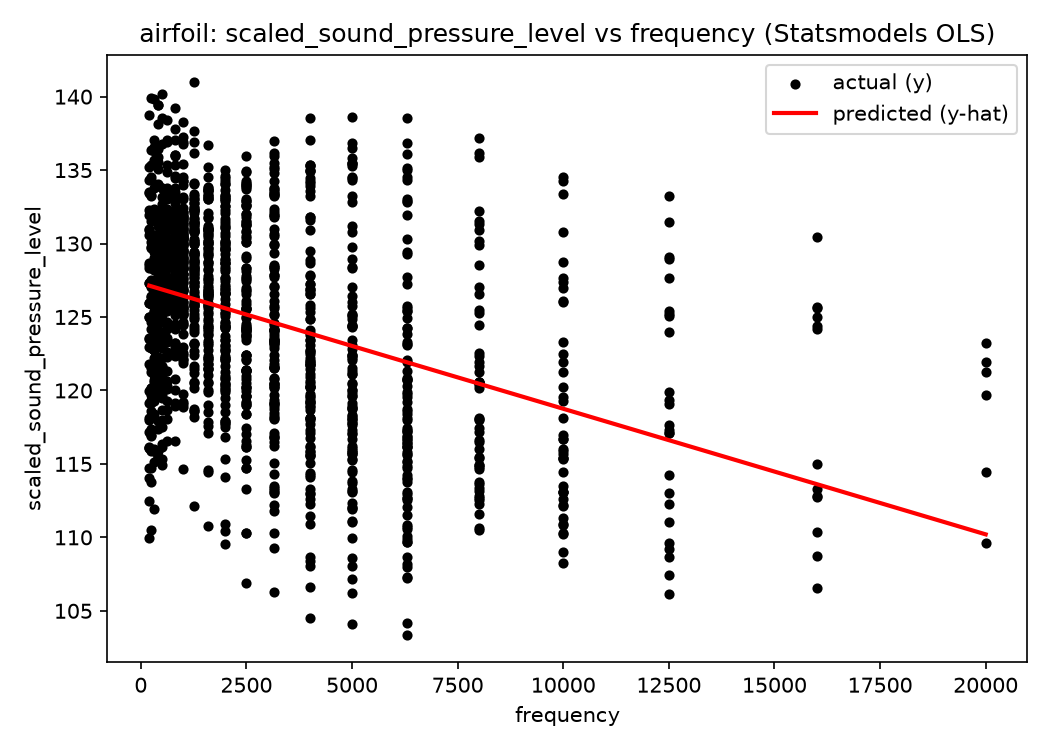
\includegraphics[width=\textwidth]{fit_vs_actual_frequency.png}
        \caption{Statsmodels}
    \end{subfigure}
    \begin{subfigure}{0.48\textwidth}
        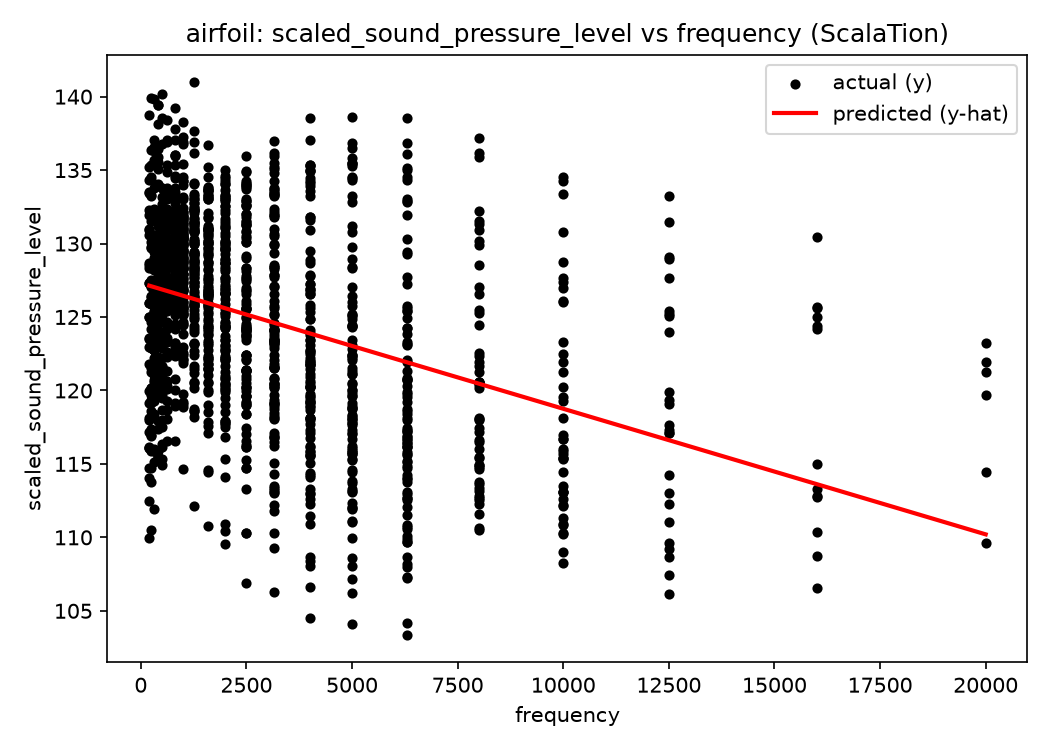
\includegraphics[width=\textwidth]{scalation_fit_vs_actual_frequency.png}
        \caption{ScalaTion}
    \end{subfigure}
    \caption{Sound pressure level vs.\ frequency: actual (black) and predicted (red) values.}
\end{figure}

\subsubsection*{Feature: suction\_side\_displacement\_thickness}
\textbf{ScalaTion fit report:}
\lstinputlisting{listings/airfoil_suction_side_displacement_thickness_scalation.txt}

\textbf{Statsmodels fit report:}
\lstinputlisting{../results/airfoil/ols_summary_suction_side_displacement_thickness.txt}

\textbf{Summary statement:} Both tools agree exactly on
$\hat{y} = 126.6632 - 164.0275\,x$. Each additional meter of suction-side
displacement thickness is associated with a decrease of about 164 dB in
sound pressure level (this feature ranges only from about 0.0004 to 0.058
m, so realistic changes correspond to a few dB); the model explains only
9.8\% of the variance ($R^2=0.0978$, adj.\ $R^2=0.0972$), though the slope
is highly statistically significant ($F=162.64$, $p<0.001$).

\begin{figure}[H]
    \centering
    \begin{subfigure}{0.48\textwidth}
        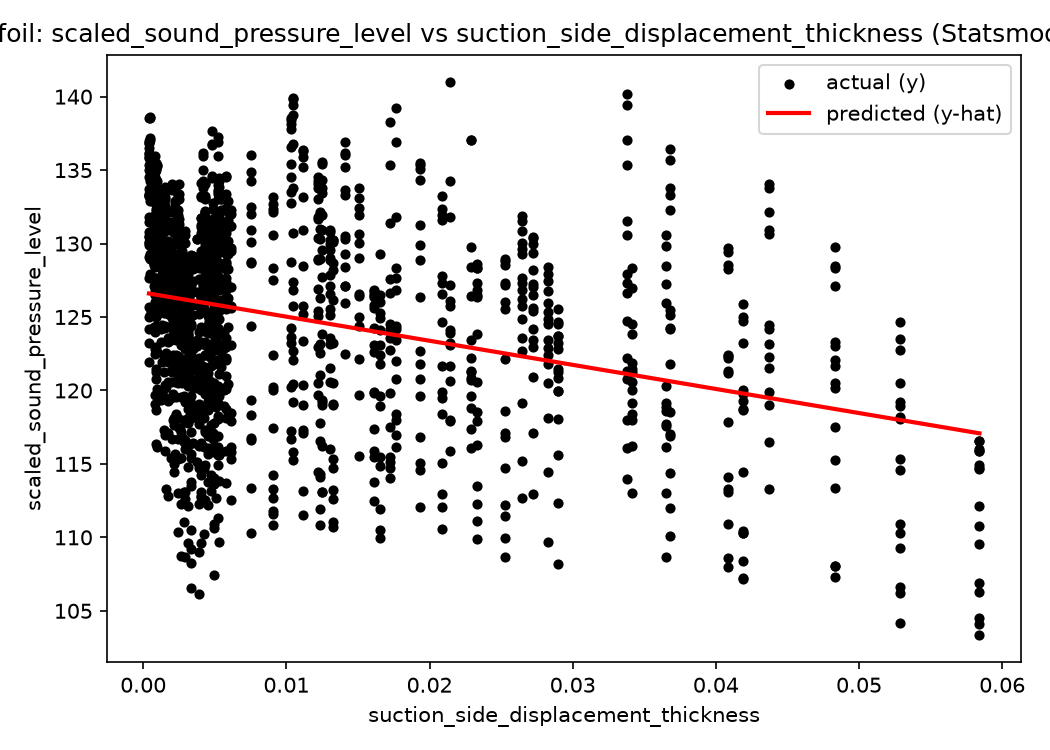
\includegraphics[width=\textwidth]{fit_vs_actual_suction_side_displacement_thickness.png}
        \caption{Statsmodels}
    \end{subfigure}
    \begin{subfigure}{0.48\textwidth}
        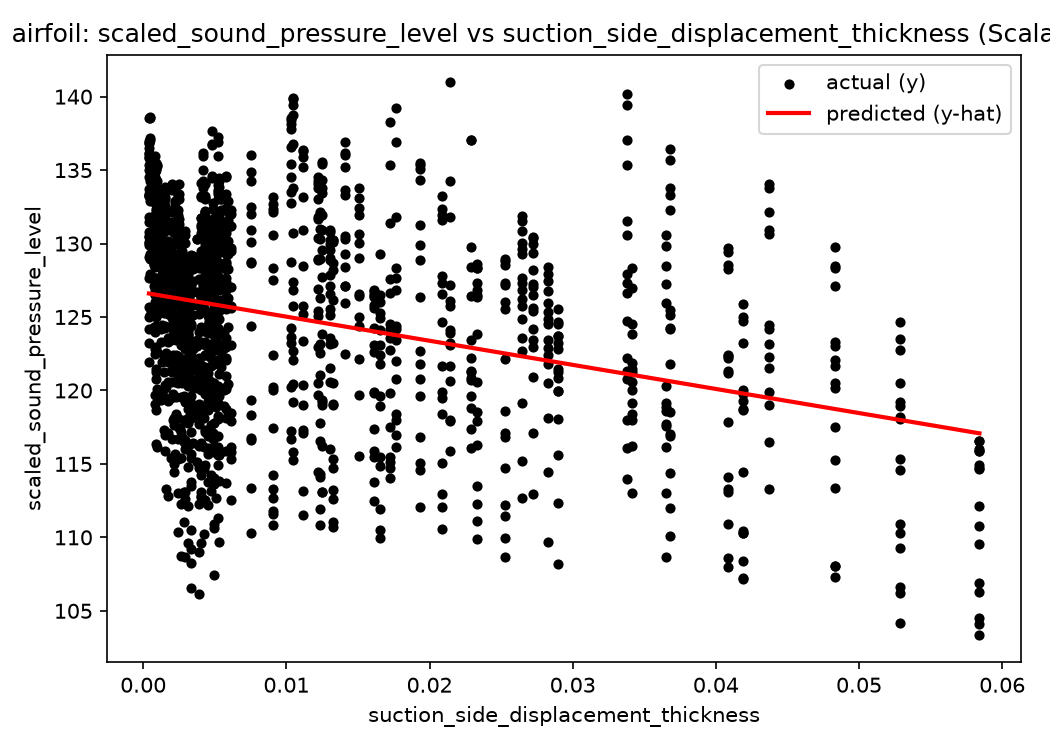
\includegraphics[width=\textwidth]{scalation_fit_vs_actual_suction_side_displacement_thickness.png}
        \caption{ScalaTion}
    \end{subfigure}
    \caption{Sound pressure level vs.\ suction-side displacement thickness: actual (black) and predicted (red) values.}
\end{figure}

\subsection{Discussion}
Of the three datasets studied, Airfoil Self-Noise shows the weakest linear
relationships: even the best single predictor, \texttt{frequency}, explains
only about 15\% of the variance in sound pressure level, and the boundary-
layer \texttt{suction\_side\_displacement\_thickness} feature explains under
10\%. Both relationships are negative and statistically significant, but the
low $R^2$ values and the wide scatter in the fit plots indicate that
aerodynamic self-noise is driven by a more complex, likely nonlinear and
multivariate interaction of frequency, angle of attack, geometry, and flow
velocity -- consistent with the physics of turbulent boundary-layer noise
generation, which does not vary linearly with any single parameter. This
dataset would likely require a nonlinear or multiple-regression model (or the
neural-network approaches used in the original NASA study) to achieve strong
predictive accuracy.

\clearpage
\section*{Cross-Dataset Summary}
\begin{itemize}
    \item \textbf{Auto MPG}: strongest simple-regression fit of the three
    ($R^2 \approx 0.69$ for \texttt{weight}); vehicle size/mass is a good
    linear proxy for fuel economy.
    \item \textbf{Concrete}: moderate fit ($R^2 \approx 0.25$ for
    \texttt{cement}); strength is inherently multivariate.
    \item \textbf{Airfoil}: weakest fit ($R^2 \approx 0.15$ for
    \texttt{frequency}); self-noise generation is a complex, nonlinear
    aerodynamic phenomenon poorly captured by any single linear predictor.
\end{itemize}
In every case, ScalaTion's \texttt{SimpleRegression} and Python's Statsmodels
\texttt{OLS} produced numerically identical coefficients and $R^2$ values,
confirming both implementations solve the same least-squares problem
correctly.

\end{document}
